%\documentclass[acmsmall, screen, review, anonymous]{acmart}
\documentclass[acmsmall, screen]{acmart}

% Revision cover letter: https://docs.google.com/document/d/1ue1zHnTmnHmwwDP7-8p7e6VPajfB8ByVkpvCwhd0Mdc/edit?tab=t.0

\usepackage{syntax}
\usepackage{booktabs} % For formal tables
\usepackage{mathtools}
\usepackage{forest}
\usepackage{subcaption}
\usepackage[ruled]{algorithm2e} % For algorithms
\usepackage{svg} % For svg images
\usepackage{fancyvrb}
\usepackage{cleveref}

\usepackage{tikz}
\renewcommand{\algorithmcfname}{ALGORITHM}
\SetAlFnt{\small}
\SetAlCapFnt{\small}
\SetAlCapNameFnt{\small}
\SetAlCapHSkip{0pt}
\IncMargin{-\parindent}


% Metadata Information
%\acmJournal{TWEB}
%\acmVolume{9}
%\acmNumber{4}
%\acmArticle{39}
%\acmYear{2010}
%\acmMonth{3}
%\copyrightyear{2009}
%\acmArticleSeq{9}

% Copyright
%\setcopyright{acmcopyright}
%\setcopyright{acmlicensed}
%\setcopyright{rightsretained}
%\setcopyright{usgov}
%\setcopyright{usgovmixed}
%\setcopyright{cagov}
%\setcopyright{cagovmixed}

% DOI
%\acmDOI{0000001.0000001}

% Paper history
%\received{February 2007}
%\received[revised]{March 2009}
%\received[accepted]{June 2009}

\usepackage{xcolor}
\newcommand{\todo}[1]{\textcolor{red}{TODO: #1}\PackageWarning{TODO:}{#1!}}

%%% The following is specific to PLDI '25 and the paper
%%% 'Spineless Traversal for Layout Invalidation'
%%% by Marisa Kirisame, Tiezhi Wang, and Pavel Panchekha.
%%%
\setcopyright{cc}
\setcctype{by}
\acmDOI{10.1145/3729322}
\acmYear{2025}
\acmJournal{PACMPL}
\acmVolume{9}
\acmNumber{PLDI}
\acmArticle{219}
\acmMonth{6}
\received{2024-11-15}
\received[accepted]{2025-03-06}

% Document starts
\begin{document}

\title{Spineless Traversal for Layout Invalidation}

\author{Marisa Kirisame}
\orcid{0000-0002-3418-4835}
\affiliation{%
  \institution{University of Utah}
  \city{Salt Lake City}
  \country{USA}
}
\email{marisa@cs.utah.edu}

\author{Tiezhi Wang}
\orcid{0009-0003-7002-6011}
\affiliation{%
  \institution{Tongji University}
  \city{Shanghai}
  \country{China}
}
\email{2152591@tongji.edu.cn}

\author{Pavel Panchekha}
\orcid{0000-0003-2621-3592}
\affiliation{%
  \institution{University of Utah}
  \city{Salt Lake City}
  \country{USA}
}
\email{pavpan@cs.utah.edu}

\begin{abstract}
Latency is a major concern for web rendering engines
  like those in Chrome, Safari, and Firefox.
These engines reduce latency by using
  an \emph{incremental layout algorithm}
  to redraw the page when
  the user interacts with it.
In such an algorithm,
  elements that change frame-to-frame are marked dirty, and
  only those elements are processed
  to draw the next frame,
  dramatically reducing latency.
However, the standard incremental layout algorithm
  must search the page for dirty elements,
  accessing auxiliary elements in the process.
These auxiliary elements
  add cache misses and stalled cycles,
  and are responsible for a sizable fraction
  of all layout latency.

We introduce a new, faster incremental layout algorithm
  called Spineless Traversal.
Spineless Traversal
  uses a cache-friendlier priority queue algorithm
  that avoids accessing auxiliary nodes
  and thus reduces cache traffic and stalls.
This leads to dramatic speedups
  on the most latency-critical interactions
  such as hovering, typing, and animation.
Moreover, thanks to numerous low-level optimizations,
  Spineless Traversal is competitive
  across the whole spectrum of incremental layout workloads.
Spineless Traversal is faster than the standard approach
  on \PctFaster of \NumFrames~benchmarks,
  with a mean speedup of \MeanSpeedup
  concentrated in the most latency-critical interactions.
\end{abstract}

\newcommand{\DBPQoverheadCount}{2216}
\newcommand{\DBPQoverheadpctslowdown}{21.8\%}
\newcommand{\DBPQoverheadpctspeedup}{78.2\%}
\newcommand{\DBPQoverhead}{\ensuremath{3.23\times}\xspace}
\newcommand{\DBPQeval}{0.99}
\newcommand{\DBPQtotal}{\ensuremath{1.78\times}\xspace}
\newcommand{\DBPQsmalloverheadCount}{1346}
\newcommand{\DBPQsmalleval}{0.99}
\newcommand{\DBPQsmalltotal}{\ensuremath{2.35\times}\xspace}
\newcommand{\DBPQlargeoverhead}{1.29}
\newcommand{\DBPQlargeeval}{0.99}
\newcommand{\DBPQlargetotal}{1.17}
\newcommand{\TotalDiffCount}{2216\xspace}
\newcommand{\TotalTraceCount}{50\xspace}

\newcommand{\NumWebsites}{\TotalTraceCount}
\newcommand{\NumFrames}{\TotalDiffCount}
\newcommand{\MeanSpeedup}{\DBPQtotal}
\newcommand{\MeanSpeedupSmall}{\DBPQsmalltotal}
\newcommand{\PctSlower}{25.14\%\xspace}
\newcommand{\PctFaster}{74.86\%\xspace}
\newcommand{\PctSmall}{60.7\%\xspace}


%
% Generate CCS codes using http://dl.acm.org/ccs.cfm and paste below
%
\begin{CCSXML}
<ccs2012>
   <concept>
       <concept_id>10011007.10011006.10011041.10011047</concept_id>
       <concept_desc>Software and its engineering~Source code generation</concept_desc>
       <concept_significance>500</concept_significance>
       </concept>
   <concept>
       <concept_id>10011007.10011006.10011041.10011046</concept_id>
       <concept_desc>Software and its engineering~Translator writing systems and compiler generators</concept_desc>
       <concept_significance>500</concept_significance>
       </concept>
   <concept>
       <concept_id>10011007.10011006.10011050.10011017</concept_id>
       <concept_desc>Software and its engineering~Domain specific languages</concept_desc>
       <concept_significance>500</concept_significance>
       </concept>
   <concept>
       <concept_id>10003752.10003809</concept_id>
       <concept_desc>Theory of computation~Design and analysis of algorithms</concept_desc>
       <concept_significance>500</concept_significance>
       </concept>
 </ccs2012>
\end{CCSXML}

\ccsdesc[500]{Software and its engineering~Source code generation}
\ccsdesc[500]{Software and its engineering~Translator writing systems and compiler generators}
\ccsdesc[500]{Software and its engineering~Domain specific languages}
\ccsdesc[500]{Theory of computation~Design and analysis of algorithms}
%
% End generated code
%

% We no longer use \terms command
%\terms{Design, Algorithms, Performance}

\keywords{Web Browsers, Layout, Incremental Computing, Order Maintenance, Latency}

\maketitle

% The default list of authors is too long for headers}
\renewcommand{\shortauthors}{Marisa Kirisame, Tiezhi Wang, and Pavel Panchekha}
\section{Introduction}

Latency is a major concern for modern web rendering engines.
A rendering engine, such as that in Chrome, Firefox, or Safari,
  must redraw pages 60 times per second
  to guarantee smooth animations, fluid interactions,
  and responsive web applications.
When this frame rate cannot be met,
  the user experiences lag and may be forced to use another web application, browser, or device.
Modern 120\,Hz displays demand even lower latency.

Layout is a key driver of web rendering latency.
Layout means calculating the size and position
  of each element on the web page,
  after which the page can be rendered as pixels on the screen.
Every time the user interacts with the web page
  by hovering over an element,
  receiving updated data,
  or even observing an animation,
  the web page changes
   and must be re-laid-out.
Since layout is only one part of the larger rendering pipeline,
  this re-layout must be completed in a millisecond or less
  in order to meet the 60 frame-per-second goal.
On such a tight budget, every cycle counts!

\paragraph{Incrementalization}
The key optimization that makes this possible
  is \emph{incrementalization}.
When an element on the page changes,
  the browser \emph{marks} it dirty.
When the page is re-laid-out,
  the rendering engine traverses the page
  to find and re-lay-out only the dirty elements.
That might mark additional elements dirty,
  due to dependencies between elements,
  but typically---in, say, animations---%
  only a few nodes are ultimately re-laid-out.
In these cases, searching the tree
  for dirty elements is the bottleneck,
  especially since every element access
  is likely to incur a cache miss.

Browsers use the ``Double Dirty Bit'' algorithm
  to find dirty nodes more quickly~\cite{wbe,tali-garseil}.
This algorithm adds summary bits
  to identify and skip subtrees without any dirty elements.
While this reduces the search time,
  Double Dirty Bit still has to traverse the tree,
  starting from the root, to find dirty elements,
  and thus accesses not only the actually-dirty elements
  but many extra ``auxiliary nodes''.
On large pages,
  auxiliary nodes can significantly outnumber
  the actually-dirty elements;
  and since each node access can cause a cache miss,
  simply traversing these auxiliary nodes,
  just to check their summary bits,
  can stall the layout algorithm for hundreds of microseconds.
This problem is widely observed in practice;
  Google's widely-used web performance tool, Lighthouse,
  measures tree depth and maximum children count
  precisely because these parameters
  determine the number of auxiliary nodes.

\paragraph{Spineless Traversal}

We introduce \textit{Spineless Traversal}:
  a new, faster algorithm for incremental layout.
Unlike Double Dirty Bit,
  Spineless Traversal accesses only dirty elements,
  not auxiliary nodes.
It therefore reduces cache misses.
Spineless Traversal works by
  storing the set of dirty elements in a queue
  and jumping directly from one to the next,
  with no auxiliary nodes in between.

The key challenge is traversing the dirty nodes in the correct order. 
Recomputing a field on one node
  can mark fields on other nodes dirty,
  and the set of transitive dependencies is complex.
Fields must therefore be recomputed in a specific order,
  and Spineless Traversal must respect that order
  as it jumps from node to node.
Spineless Traversal thus stores
  a timestamp on each node,
  and uses a priority queue to traverse nodes
  in timestamp order.
To maintain timestamps as nodes are added and removed,
  Spineless Traversal \emph{order maintenance},
  which compute relative timestamps in a flexible way.
Both the priority queue and order maintenance structure
  are heavily optimized to make them competitive with Double Dirty Bit.

\paragraph{Implementation}

We implement Spineless Traversal in Megatron,
  a new compiler for incremental layout algorithms.
Megatron implements decades of research on attribute grammars:
  it statically analyzes the dependency graph,
  synthesizes recomputation and marking functions,
  and guarantees a correct incremental layout.
It implements standard optimizations
  (unboxing, interning, field packing, and jump tables)
  and compiles layout algorithms to highly efficient C++ code.
Megatron supports both Double Dirty Bit and Spineless Traversal
  via a common invalidation traversal interface,
  allowing an apples-to-apples comparison between them.

We compare the two algorithms on
  a significant fragment of web layout that includes
  line breaking, flex-box, intrinsic sizes, and many other features,
  benchmarking \TotalTraceCount real-world web pages
  like Twitter, Discord, Github, and Lichess.
Across \TotalDiffCount frames,
  Spineless Traversal is \DBPQtotal times faster on average.
Speedups are concentrated in the most latency-critical frames:
  on the \PctSmall of frames
  where at most 1\% of fields are recomputed,
  Spineless Traversal achieves a speedup
  of \MeanSpeedupSmall.

\section{Web Layout Background}

Complex
  web (Facebook, Amazon, GMail),
  desktop (VS Code, Figma, Slack),
  and mobile (WeChat) applications
  involve two software components:
  the application itself and the browser.
The application-level code, typically in JavaScript,
  implements the actual application logic and
  interacts with the browser by making DOM API calls
  that modify the browser's internal representation of the web page.
The browser then executes its ``rendering pipeline''---%
  event handling, hit testing, matching, styling,
  layout, paint, layerizing, rastering, and drawing---%
  which reads this internal representation and transforms it,
  step by step, into pixels on the screen.
Most execution time is typically spent in application code,
  but that code's effects are ultimately visible to the user
  only through ``system calls'' serviced by browser-level code.
For the application to be responsive and smooth,
  those calls have to be serviced
  in 16 milliseconds (60 frames per second).

Concretely, a browser application is written in HTML,
  which defines a tree called the ``document'',
  whose nodes include text, buttons,
  and structural elements like \texttt{div}s.
The application code binds specific callback functions
  to user actions like clicking on a button,%
  \footnote{Callbacks can also run in response to
    timers, network requests, or a dizzying array of
    other events.}
  and these callbacks can modify the HTML using DOM methods
  like \texttt{appendChild} or \texttt{setAttribute}.
When the callback finishes executing,%
\footnote{Or after multiple callbacks finish executing,
  as decided by the browser's task scheduler.}
  the browser executes the full rendering pipeline
  to display the results to the user.
Also, some DOM methods like
  \texttt{getBoundingRect} or \texttt{offsetX}
  read state computed during the rendering pipeline;
  calling these methods can requires the browser
  to perform additional passes through the rendering pipeline.
This is necessary for some common interactions like tooltips.

\subsection{The Layout Phase}
\begin{figure}
\includegraphics[scale=0.3]{tree.png}
\caption{The DOM tree for \texttt{google.com}, with 842 total nodes, a maximum fanout of 16, and a maximum depth of 18. The node marked red is part of the auto-complete suggestion box. The node color corresponds to the Double Dirty Bit algorithm, with gold representing auxiliary nodes and gray representing skipped nodes. Auxiliary nodes are a large fraction of the page even when only one node is (transitively) dirtied.
}
\label{fig:google}
\end{figure}

This paper is specifically concerned with the layout phase,
  a long-term focus of the programming languages community.
The layout phase traverses an intermediate structure
  called the ``layout tree'' and computes, for each node,
  a set of ``layout fields''
  including each element's size and position.
This computation proceeds in several passes,
  first computing intermediate layout fields
  like intrinsic width and height
  and current line ascent/descent
  before computing size and position.

The layout tree is basically the HTML tree,
  with minor differences for
  ``generated content'' (like bullets for list items)
  and ``fragmentation'' (like line breaking)
  that are not critical to this paper.
The trees are both big and unbalanced;
  the famously minimal Google home page page, for example,
  has 842 nodes, with a maximum fanout of 16 and depth of 18;
  it is drawn in \Cref{fig:google}.
In memory, the layout tree is stored as a pointer tree,
  with the children of each node stored in a doubly-linked list.%
\footnote{
This ensures that node insertions and deletions are fast,
  even in poorly-balanced trees.
}
The application can add or remove nodes from this tree,
  or write to their ``properties'' and ``attributes'',
  to update what the user sees.

Each node's layout fields depend on the layout fields
  of its neighbors.
For example, imagine a paragraph containing several lines;
  there would be a layout node for the paragraph
  and another for each line as children of the paragraph's.
The height of the paragraph, in this case,
  would be the sum of the heights of all its children
  plus any gaps between them,
  while a line's width would be its parent's width,
  minus some padding.
Of course, real-world web layout is much more complex;
  Chrome's implementation is about 100,000 lines of code
  and computes hundreds of fields per node.
To compute all these fields correctly, the layout algorithm
  recursively traverses the tree multiple times.
For example, the layout algorithm might first compute
  the intrinsic size of each element in a bottom-up traversal;
  then compute preferred sizes, in a top-down traversal;
  and then apply flexible sizing rules in a bottom-up traversal
  to finally compute each element's actual size.
Note that not only are multiple passes necessary,
  but that each pass must visit the nodes of the layout tree
  in a specific order so that each layout field's dependencies
  are satisfied.

\begin{figure}
    \centering
    \includegraphics[width=\linewidth]{profile.png}
    \caption{
      A trace of nine milliseconds of Chrome opening Youtube;
        time flows left to right while the call stack grows down.
      The violet ``recalculate style'' and ``layout'' blocks
        are phases of the browser rendering pipeline,
        with layout in total consuming four milliseconds;
        the faint vertical lines are half-millisecond marks.
      Layout happens multiple times in one frame
        due to ``forced reflows''.
      The ``Summary'' tab at the bottom shows
        that the selected (longest) layout
        only updates 23 of 2\thinspace301~nodes
        in the layout tree.}
    \label{fig:profile}
\end{figure}

\Cref{fig:profile} shows layout performance in practice:
  a trace of Google Chrome opening YouTube,
  captured and visualized using Chrome's ``Performance'' tools.
The trace covers 9~milliseconds of execution time,
  with time running left to right.
Function calls grow downward, and the leaves,
  labeled ``recalculate style'', ``layout'',
  and ``pre-paint'' (barely visible)
  are different phases of the rendering pipeline;
  the application-level code is offscreen to the left.
In these nine milliseconds,
  the application requests layout four times
  by calling APIs that require (``forced reflow'')
  multiple passes through the rendering pipeline.
These four layouts each take longer than
  the browser developers' target latency.

Below the trace, the ``Summary'' tab shows
  more information about a single, selected layout
  taking 2.1~milliseconds.
This layout operates
  on a layout tree of 2\thinspace301~nodes,
  starting from the root of the web page (\texttt{\#document}).
However, it only needed to update 23~of~them;
  in other words, this layout was incremental.
The long running time of the layout phase
  nonetheless caused unacceptable latency;
  in fact, this frame ``drops'',
  meaning the browser isn't able to update the page
  in time to show smooth animations and interactions.

\subsection{Formal Modeling}

Luckily, the programming languages community
  has developed a sophisticated understanding of layout.
Early work by Meyerovich and others%
  ~\cite{meyerovich-1,meyerovich-2,meyerovich-3}
  developed ``attribute grammars'' as a formalism
  for defining layout rules and implementations.
The later Cassius project~\cite{cassius-1,cassius-2,cassius-3}
  developed a full, standards-compliant implementation
  of a significant fragment of web layout in this formalism,
  and the \textsc{Hecate} and \textsc{Medea}
  tools~\cite{yufeng-1,yufeng-2}
  have shown that automatic synthesis can be scaled
  to such fragments.  

\begin{figure}
\begin{align*}
\text{Layout} &\coloneq  \text{Rule}^+; \textbf{schedule}\:\text{Pass}_n^+ \\
\text{Rule} &\coloneq
  \mathbf{def}\:\text{Pass}_n()\:\{\:
    A^+;\:
    \mathsf{children}.\mathsf{forEach}(\text{Pass}_n);\:
    A^+;\:
  \} \\
A \in \text{Assignment} &\coloneq
  \text{self}.V \leftarrow T \\[4pt]
T \in \text{Term} &\coloneq
  \text{if}\ T\ \text{then}\ T\ \text{else}\ T \mid
  F(T^+) \mid
  N? \mid
  N.V \mid
  \mathsf{attribute}[V] \mid
  \mathsf{property}[V] \\
N \in \text{Neighbor} &\coloneq
  \mathsf{self} \mid \mathsf{prev} \mid
  \mathsf{next} \mid \mathsf{parent} \mid
  \mathsf{first} \mid \mathsf{last} \\[4pt]
V \in \text{Variable} &\coloneq \text{layout fields} \quad\quad
F \in \text{Function} \coloneq \text{primitive functions}
\end{align*}
\caption{
  A minimal DSL for defining web layout
    as a set (\textsf{rules}) of passes
    performed in a specific order (\textsf{schedule}).
  The syntax $P^+$ represents a sequence of non-terminal $P$.
  Passes are in-order traversals of the layout tree
    performing a sequence of assignments to local fields
    while accessing fields of the current node or its neighbors.
}
\label{fig:dsl}
\end{figure}

\Cref{fig:dsl} defines an attribute grammar.
An attribute grammar is defined by
  a set of passes (the rules)
  performed in a certain order (the schedule).
Each pass performs a recursive, in-order traversal of the tree,
  computing some fields pre-order and some fields post-order;
  every field is written to exactly once in exactly one pass.
For each field assignment $\mathsf{self}.V \gets T$,
  the expression $T$ can refer
  to fields of $\mathsf{self}$ or
  to fields of its $\mathsf{parent}$,
  $\mathsf{prev}$ and $\mathsf{next}$ sibling,
  or $\mathsf{first}$ and $\mathsf{last}$ child;
  expressions can also test whether a given neighbor
  exists ($\mathsf{N?}$).
Computations can also refer to
  attributes or properties of the current node
  using $\mathsf{attribute}[x]$ or $\mathsf{property}[x]$.%
\footnote{
HTML attributes and CSS properties
  use two different namespaces
  because some names, like \texttt{height},
  appear in both sets; there is no other semantic difference.
Other accessible properties,
  such as the tag name or image width and height
  are modeled in our implementation as special properties.
}
All computations besides field assignments are pure,
  there are no other loops or data structures,
  and the only field access allowed is to a node's neighbors.
Despite this, even complex layout features
  like flexible box layout are expressible in such a DSL.

\begin{figure}
\begin{minipage}[b]{0.68\linewidth}
\begin{align*}
& \mathbf{def}\:\text{Pass}_1()\:\{ \\
& \quad \mathsf{self}.W \gets
        \mathbf{if}\:\mathsf{parent}?\:
        \mathbf{then}\:\operatorname{max}(0, \mathsf{parent}.W - 10)\:
        \mathbf{else}\:50; \\
& \quad \mathsf{children}.\mathsf{forEach}(\text{Pass}_1); \\
& \quad \mathsf{self}.H \gets
        \mathbf{if}\:\mathsf{last}?\:
        \mathbf{then}\:\mathsf{last}.HA + 10\:
        \mathbf{else}\:\mathsf{self}.\text{attribute}[\mathsf{height}]; \\
& \quad \mathsf{self}.HA \gets
        \mathbf{if}\:\mathsf{prev}?\:
        \mathbf{then}\:\mathsf{prev}.HA + \mathsf{self}.H + 5\:
        \mathbf{else}\:\mathsf{self}.H; \\
& \} \\
& \mathbf{schedule}\:\text{Pass}_1
\end{align*}
\caption{
  A minimal paragraph layout implementation,
    computing width $W$ and height $H$,
    with 5 pixels padding and 5 pixel gaps between lines.
  The intermediate $HA$ field sums the height
    of a node and all its previous siblings and gaps.
  This simple layout algorithm has one pass,
    but real-world layouts contain multiple.
}
\label{fig:layout-simple}
\end{minipage}\hfill%
\begin{minipage}[b]{0.28\linewidth}
\centering
\includegraphics[width=\linewidth,trim=0 0 11in 0,clip]{LayoutExample.pdf}
\caption{The layout algorithm running on a layout tree of size 4. All nodes have an height attribute of 10.
}
\end{minipage}
\end{figure}
\Cref{fig:layout-simple} shows
  example layout rules for paragraphs and lines,
  defined using an attribute grammar.
Here the nodes for paragraphs and lines have three layout fields:
  a width $W$, a height $H$, and an intermediate field $HA$
  that computes the height of a node and its previous siblings
  (plus any gaps between lines).
Width information propagates from parents to children,
  starting at 50 pixels and subtracting, at each level,
  5 pixels of padding on the left and right.
Height information propagates from children to parents---%
  a node's height is the sum of its children's heights,
  plus 5-pixel gaps between lines---%
  and relies on the intermediate $HA$ field
  which propagates information from previous to next siblings.
Note that the idea of ``summing all children's heights''
  is not expressed with a loop;
  instead, it is expressed as the additional $HA$ layout field,
  which has its own computation rule.

Attribute grammar DSLs can be heavily optimized.
The layout fields can stored in the node itself,
  tightly packed to ensure locality.
Computations can use primitive data types
  like integers, floats, and enumerations;
  strings can be interned and hash tables statically flattened.
The only pointer accesses are to neighboring nodes,
  which are likely to be in cache.
Branch mis-prediction are relatively rare
  given the minimal control flow.
The tree structure itself does not change \emph{during layout}.
This efficiency is critical to browser developers.

A key property of attribute grammar DSLs like this one
  is that dependencies and traversal orders are static.
Specifically, for any field assignment,
  examining the expression $T$ reveals
  which other fields on which other nodes it depends on.
These static dependencies are critical for invalidation.
Also, the schedule language ensures that
  the relative order in which two fields are computed
  never changes, even as nodes are added or removed.
This is critical for Spineless Traversal.
In this paper, we assume
  that the rules have no cyclic dependencies
  and that the schedule
  respects field dependencies;
  we also assume that the schedule has already been optimized
  by fusing traversals and ordering field assignments.
A substantial literature exists on these topics~%
  \cite{grafter,yufeng-1,yufeng-2};
  the layout implementation in our evaluation
  is detailed in Section~\ref{sec:layout-impl}.
In any case, while this paper focuses on web layout,
  we expect Spineless Traversal to be applicable
  to incremental computations in other domains,
  including in compilation, static analysis,
  computer graphics, and databases,
  as long as they can be expressed as an attribute grammar
  in this or a similar DSL.
\section{Incremental Layout}

An \emph{incremental} layout algorithm
  reuses layout field values between layouts when possible.
For example, when the user moves their mouse,
  a tooltip may need to move to follow the cursor;
  incremental layout would re-compute the position of the tooltip
  while reusing all other layout fields for all other elements.
Most layouts change only a small fraction of fields---%
  especially the most latency-critical interactions
  like hovers, drags, animations, and text editing---%
  so incremental layout can be dramatically faster
  than computing each layout from scratch.

\subsection{Dirty Bits}
\label{sec:recompute-phase}

Incremental layout is conceptually straightforward. 
Each layout field has a corresponding \textit{dirty} bit,
  which defines whether that layout field needs to be recomputed.%
\footnote{\emph{Packed} layout fields can all have
  the same corresponding dirty bit,
  which is set if any of those fields need to be recomputed.}
APIs that write to an attribute or property,
  or add or remove layout nodes,
  set the dirty bits for all layout fields
  that read from those fields or node pointers.
For example,
  in the paragraph layout of \Cref{fig:layout-simple},
  when a node's \textsf{height} attribute is changed,
  its $H$ field must be marked dirty.
When a subtree is deleted,
  its next sibling's $HA$ field must be marked dirty.
If the subtree was the last child of its parent,
  the parent's $H$ field must also be marked dirty.
This set of fields can be statically determined in our DSL
  and in fact our Megatron compiler synthesizes
  this marking code automatically.

Incremental layout then has the task of clearing dirty bits
  by recomputing dirty fields.
Conceptually this is simple:
  find all dirty bits on all nodes and recompute
  the fields they correspond to.
However, when a layout field is recomputed,
  its value might change,
  and then any layout fields that read the old value
  are would be out of date.
Thus, when incremental layout modifies a layout field,
  it must dirty all layout fields that depend on it,
  ``propagating'' dirty bits through the document.
For example,
  in the paragraph layout of \Cref{fig:layout-simple},
  when a node's $H$ field is recomputed,
  its $HA$ field must be marked dirty.
When that $HA$ field is recomputed,
  its next sibling's $HA$ field is then marked dirty in turn.
Because of dirty bit propagation,
  the set of layout fields \emph{currently} marked dirty
  is distinct from the set of all layout fields
  that incremental layout must ultimately recompute.

This second set is \emph{discovered}
  in the process of performing incremental layout:
  dirty bits are only propagated
  when a layout field's value changes,
  which is only known when that field is recomputed
  and the old and new value can be compared.
For example, suppose the user is typing out a paragraph of text,
  laid out using \Cref{fig:layout-simple}'s layout algorithm.
Most edits just add text to a single line,
  not affecting its height or available width;
  these only end up dirtying a single field on a single node.
This is why incremental layout works:
  many interactions---%
  especially latency-critical ones like
  hovers, drags, animations, and text editing---%
  do not change fields on containing elements,
  and end up affecting only a small portion of the page.

\subsection{Recomputation Order}

Incremental layout strives to minimize
  the number of layout fields recomputed.
That requires ensuring that, once recomputed,
  a layout field is not marked dirty again during that layout.
Luckily, there is a simple way to guarantee this:
  a correct from-scratch layout
  always processes a field's dependencies before the field itself,
  so recomputing layout fields
  in the \emph{same relative order} as a from-scratch layout
  ensures that each layout field is marked dirty at most once.
A naive incremental layout algorithm might thus
  execute the same layout schedule as a from-scratch layout
  but skip re-computing any fields that aren't dirty.
This algorithm recomputes the minimal number of layout fields,
  clears all the dirty bits,
  and avoids ever recomputing a layout field more than once.

However, this naive algorithm isn't particularly fast:
  it must access every layout node to check its dirty bits,
  which incurs a lot of cache misses.
In the common case, most dirty bits aren't set;
  these ``auxiliary'' accesses cause needless cache misses
  and end up wasting a significant fraction of run time.
For incremental layout to be fast,
  auxiliary accesses---%
  accesses that don't result in field recomputations---%
  must be minimized.

\subsection{The Double Dirty Bit Algorithm}

The state-of-the-art Double Dirty Bit algorithm
  uses summary bits to reduce auxiliary accesses;
  it is used, with variations, in all major rendering engines.
For each dirty bit, we add a second ``summary bit'',
  which is set for any node where the corresponding dirty bit
  is set anywhere in the \emph{subtree} rooted at that node.
When a field is marked dirty, its dirty bit is set,
  and the associated summary bit is also set
  on that node and all its ancestors.
When performing incremental layout,
  subtrees whose summary bits are clear can be skipped.
Figure~\ref{fig:find-dirty-nodes} contains
  pseudo-code for Double Dirty Bit
  as an iterator over dirty nodes.

\begin{figure}
\begin{minipage}[b]{0.5\linewidth}
\begin{verbatim}
def mark_dirty(self):
    self.dirty_bit = True
    self.set_summary_bit()

def set_summary_bit(self):
    if self.summary_bit: return
    self.summary_bit = True
    if self.parent:
        self.parent.set_summary_bit()
\end{verbatim}
\caption{Setting the summary bit for a node.}
\label{fig:set-summary-bits}
\end{minipage}\hfill%
\begin{minipage}[b]{0.5\linewidth}
\begin{verbatim}
def find_dirty_nodes(self):
    if self.dirty_bit:
        yield self
        self.dirty_bit = False
    if self.summary_bit:
        # Access auxiliary nodes
        for child in self.children:
            find_dirty_nodes(child)
        self.summary_bit = False
\end{verbatim}
\caption{Finding the dirty nodes in a tree.}
\label{fig:find-dirty-nodes}
\end{minipage}
\end{figure}

Skipping subtrees with no dirty bits
  reduces the number of auxiliary accesses
  and greatly improves performance~\cite{tali-garseil,wbe}.
However, \emph{some} auxiliary accesses remain.
Specifically, when a dirty bit is set on some node,
  summary bits will be set for all ancestors of that node,
  which Double Dirty Bit will have to check.
Moreover, for each ancestor,
  Double Dirty Bit will recurse into its children,
  adding even more auxiliary accesses.
Since layout trees are poorly balanced and often very wide,
  the number of auxiliary accesses can be large.
For example,
  a single dirtied node in \Cref{fig:google} has 66 auxiliary nodes,
  and on larger pages the dirty-to-auxiliary ratio can be even worse.

Developers can sometimes reduce the number of auxiliary accesses
  by reorganizing large, complex pages;
  performance monitoring tools
  like Google's Lighthouse~\cite{lighthouse}
  will suggest doing so.
But this can require global changes to the shape of the layout tree,
  which (in modern frameworks like React)
  requires refactoring the application as a whole.
Naturally, an invalidation algorithm that simply
  did not require so many auxiliary nodes
  would be a superior solution.
And while this is a quite specialized performance problem,
  it is a major source of latency in existing web browsers,
  which in turn are both critical application platforms
  and also already highly optimized,
  meaning remaining sources of latency are
  particularly challenging.
\section{Spineless Traversal}

Spineless Traversal is such an algorithm.
Unlike Double Dirty Bit,
  Spineless Traversal can jump directly to the next dirty node
  without accessing any auxiliary nodes;
  as a result, it suffers dramatically fewer cache misses
  than Double Dirty Bit.
Achieving this requires a more computationally-heavy approach,
  storing all dirty nodes in a priority queue
  and maintaining the correct traversal order
  using an order maintenance data structure.
Spineless Traversal's savings in cache misses
  outweigh the greater computational requirements
  of these data structures.

\subsection{The Priority Queue}

Spineless traversal is conceptually simple.
Each node field in the layout tree is assigned a label,
  indicating its position in a layout trace\ref{par:trace}.
Node fields are placed in a priority queue when dirtied,
  with the label used as their priority.
To perform an incremental layout,
  node fields are popped from the priority queue and recomputed,
  with dependent fields
  added back to the priority queue as they get dirtied,
  until the priority queue is empty.
Because the priority queue pops node fields with smaller labels first,
  Spineless Traversal respects the dependency order of layout.
Since only dirty nodes are ever pushed or popped from the priority queue,
  no auxiliary nodes are accessed.

We use a min-heap for our priority queue,
  which is cache-friendly and requires relatively few operations
  for each push and pop.
Moreover, the queue is typically small:
  while there are typically thousands of nodes,
  with each node having approximately 50 fields,
  the priority queue typically contains less than 1000 fields,
  and for the most latency-critical interactions,
  like hovers or drags, it can contain 100 or fewer.
With such a small size, a priority queue push/pop requires
  5--10 label comparisons,
  which can be performed in roughly the time
  for one or two L2 cache misses
  in our optimized implementation.
Since there are typically \emph{far} more auxiliary than dirty nodes,
  this means Spineless Traversal performs much faster
  than Double Dirty Bit.

\subsection{Order Maintenance}

The key to Spineless Traversal is maintaining the labels.
The issue is that layout nodes are added and removed over time;
  labels need to be comparable,
  but it also needs to be possible
  to add new labels between existing ones,
  arbitrarily.
Following SAC~\cite{SAC},
  spineless traversal achieves this using
  an \emph{order maintenance} data structure.
First introduced by \citet{OM},
  order maintenance is a data structure
  that maintains a totally ordered set of objects
  while allowing objects
  to be added and removed from the order arbitrarily.
Crucially, both adding/removing and comparing nodes
  takes $O(1)$ time.
Abstractly, order maintenance provides the following API:

\begin{enumerate}
\setlength{\itemindent}{8em}
  
\item[$\mathsf{Compare}(p, q)$] Decides whether $p$ or $q$ comes first in the order (or are equal).
\item[$\mathsf{Head}()$] Returns the first object of the order.
\item[$\mathsf{Create}(p)$] Creates and returns a new object right after $p$.
\end{enumerate}

\noindent
Deleting OM objects is also possible; however,
  our implementation does not.

Our implementation is based on that by \citet{SOM},
  which uses a two-level structure with
  a double-linked list of double-linked lists.
Objects are represented by nodes in the lower-level lists.
Both levels are ordered;
  the total order traverses lower-level lists in order,
  in the order dictated by the higher-level list.
Each object (node in the lower-level list)
  maintains a pointer to its higher-level list cell;
  two objects are in the same low-level list
  if they have the same higher-level pointer.
To allow fast comparisons between nodes,
  both low-level and high-level list cells store
  an unsigned integer of fixed size
  (in our implementation, 32~bits)
  called labels.
Within both lists, node labels are strictly increasing;
  this makes comparisons fast.
Specifically, comparison has two cases:
  the two objects can be in the same low-level list,
  in which case their labels can be compared,
  or in different ones, in which case
  their parents' labels can be compared.
This comparison operation is
  the bulk of the Spineless Traversal time
  so its simplicity is essential;
  Section~\ref{sec:opt} discusses how we
  micro-optimize it in our implementation.

To create an object inside an order maintenance structure,
  a new lower-level list cell is created
  whose label is the average of the two neighboring labels.%
\footnote{
  When creating a node after the last node,
  the maximum representable number is used as the larger number.
}
If the two labels differ by exactly 1, however,
  this becomes impossible (a label would be repeated).
In this case, the data structure re-balances itself,
  evenly reassigning labels to existing objects.
This process might
  create a new higher-level list cell
  to split a lower-level list in two,
  ensuring a sufficiently large gap between its cells.
Rebalancing is algorithmically tricky
  but is not a significant time sink in our use case,
  so we do not detail re-balancing here;
  details can be found in \citet{SOM}.

\begin{figure}
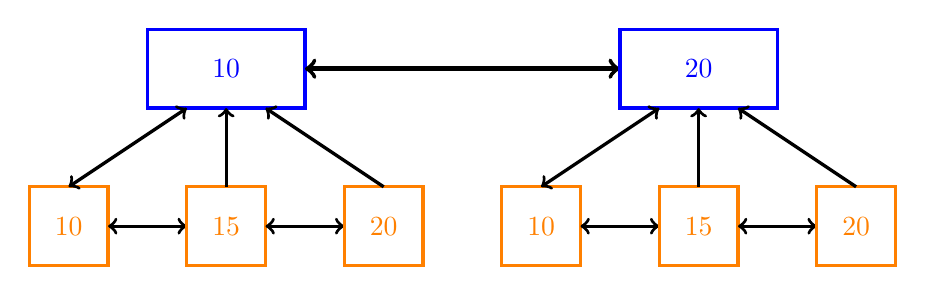
\begin{tikzpicture}
\draw[blue, very thick] (1.5,0) rectangle (3.5,1) node[pos=.5]{10};
\draw[ultra thick, <->] (3.5,0.5) -- (7.5,0.5);
\draw[blue, very thick] (7.5,0) rectangle (9.5,1) node[pos=.5]{20};

\draw[orange, very thick] (0, -2) rectangle (1,-1) node[pos=.5]{10};
\draw[very thick, <->] (0.5,-1) -- (2,0);
\draw[very thick, <->] (1,-1.5) -- (2,-1.5);
\draw[orange, very thick] (2, -2) rectangle (3,-1) node[pos=.5]{15};
\draw[very thick, ->] (2.5,-1) -- (2.5,0);
\draw[very thick, <->] (3,-1.5) -- (4,-1.5);
\draw[orange, very thick] (4, -2) rectangle (5,-1) node[pos=.5]{20};
\draw[very thick, ->] (4.5,-1) -- (3,0);

\draw[orange, very thick] (6, -2) rectangle (7,-1) node[pos=.5]{10};
\draw[very thick, <->] (6.5,-1) -- (8,0);
\draw[very thick, <->] (7,-1.5) -- (8,-1.5);
\draw[orange, very thick] (8,-2) rectangle (9,-1) node[pos=.5]{15};
\draw[very thick, ->] (8.5,-1) -- (8.5,0);
\draw[very thick, <->] (9,-1.5) -- (10,-1.5);
\draw[orange, very thick] (10, -2) rectangle (11,-1) node[pos=.5]{20};
\draw[very thick, ->] (10.5,-1) -- (9,0);

\end{tikzpicture}
\caption{An Order Maintenance data structure. The blue node represent the higher level doubly linked list, and each node store a lower level doubly linked list, denoted by the orange node. Lower level node also store a pointer to the higher level node. Each node additionally hold an unsigned integer, label, such that inside a single list the node earlier have a strictly smaller label then the node later.}
\label{fig:om}
\end{figure}

\subsection{Bulk insertion and deletion}

\label{sec:tree-insertion}
Bulk insertions into the layout tree are common,
  often due to a ``lazy loading'' pattern:
  a ``shell'' web page loads first and shows a loading indicator;
  then the ``content'' loads and is inserted into the page
  as a single large subtree.
This pattern is encouraged by frameworks like React,
  and can occur in several stages, with a ``shell''
  first inserting ``subshells'' which
  themselves load subcomponents in turn.
Efficiently inserting the large subtree
  requires special care in Spineless Traversal.

The basic issue is that all fields of all nodes in the subtree
  need to have them and their OM objects initialized,
  yet we also want subtree insertion to be fast.
Our solution adds these ``initialization passes''
  as special elements in the priority queue.%
\footnote{
  Just enqueueing all fields of all nodes in the subtree
    is not a good idea---it will create a large queue with slow queue operations.
  In our experiments, this often took the queue
    from tens to thousands of members,
    leading to a small integer slowdown.
}
In other words, the priority queue can contain
  not only $(n, v)$ pairs for a dirtied field
  but also $(r, p)$ fields pointing to the root $r$
  of an entire subtree that needs to be initialized
  for pass $p$.
When a subtree $T$ is inserted, each pass for it is enqueued;
  the Order Maintenance object for that
  is created after the OM of the last field
  initialized by $P$ in $T$'s previous sibling or parent.
In this way, we maintain the consistency of incremental layout 
  with from-scratch layout.
\footnote{
  An edge case is inserting a subtree into
    a subtree that itself has not yet been laid out.
  In this case no further actions need to be taken,
    since both subtrees will be visited together.}

When one of these $(r, p)$ elements is popped from the queue,
  the pass $p$ is performed on the whole subtree under $r$,
  creating all necessary order maintenance nodes.
Since all fields in newly-created nodes are initially dirty,
  performing this pass will not enqueue any fields
  in the priority queue,
  meaning that no priority queue operations
  need to be performed.
Likewise, since all data accesses are local,
  no existing nodes will refer to any newly-inserted node
  except the root node,
  so no nodes need to be dirtied when running $p$ on the subtree.
This means that, when initializing a subtree,
  no priority queue operations or dirty bit propagations
  need to be performed,
  which makes subtree insertion faster.
(However, order maintenance objects still need to be created,
  meaning that, despite these optimizations,
  Spineless Traversal is typically
  slower than Double Dirty Bit
  for subtree insertion.)

When deleting a subtree,
  some nodes in the subtree may
  already be in the priority queue;
  for example, this can happen if
  a subtree is inserted and then later deleted.
To avoid unnecessary recomputation,
  we add a ``deleted'' bit to each node
  and skip recomputing such node.%
\footnote{Those nodes are ref-counted and the memory will be reclaimed at the right moment.}
\section{MegaTron}

To evaluate Spineless Traversal,
  we implement it for a simplified web layout algorithm
  implemented in the DSL of Figure~\ref{fig:dsl}
  and compiled by a compile we call MegaTron.
In this section, we first describe
  the layout modes implemented,
  then how we compile the DSL to a layout engine,
  and finally compare Spinless Traversal to Double Dirty Bit
  on a collection of real-world web page interactions.

\subsection{Web Layout Algorithm}
\label{sec:layout-impl}

To compare Spineless Traversal and Double Dirty Bit,
  we needed a web layout algorithm
  that was decoupled from its invalidation strategy.
Unfortunately, existing browser rendering engines
  are too complex and too tightly coupled
  to their current invalidation strategy,
  making it impossible to reuse them.
We instead implemented our own web layout algorithm
  based on the Cassius and MEDEA formalizations%
  ~\cite{cassius-1,cassius-2,yufeng-2}.
Naturally, this implementation is simplified
  compared to a real-world web browser
  and only implements a subset of features.
However, we took care to implement several features
  with complex invalidation behavior,
  including intrinsic width, flex-box layout, and positioning.
In total, our implementation is 700 lines of code
  in a custom DSL called Megatron,
  which compute approximately 50 fields for each layout node.
The remainder of this section describes
  several key layout features implemented in our layout algorithm.

\paragraph{Box model}.
Each layout node has an $x$, $y$, width and height field.
Typically the rectangle this represents contains
    all of the node's children, while sibling elements
    don't overlap.
In general, width is computed top-down
  (children's width depend on parent's width),
  height is computed bottom-up
  (parent's height is sum of children's heights)
  and $x$ and $y$ are computed in-order.
This forms long dependency chains between elements,
    where updating one element can cause many others
    to be transitively dirtied.
However, the \texttt{width},
    \texttt{min-width}, and \texttt{max-width} CSS properties,
    and similar for \texttt{height},
    can directly set width and height,
    breaking these dependency chains.
Our layout algorithm's support for these properties
    means this early-stopping behavior is tested.
That said, even the
  explicit \texttt{width} and \texttt{height} properties
  allow ``percentage values'' like \texttt{50\%},
  which are resolved relative to the parent and thus
  still create inter-node dependencies.
	
\paragraph{Line Breaking}
Line breaking lays out inline layout nodes (text)
  horizontally from left to right,
  until the edge of the parent box is reached,
  and which point the next layout node is placed
  at the left edge of its parent,
  one line below its previous sibling.
Line breaking requires handling control dependencies,
  where one layout nodes' width may move layout nodes
  from one line to another by changing line breaking.
Additionally, our layout algorithm
  allows different lines to have different height
  (based on the height of the largest layout node in the line),
  which introduces a field (line height)
  that is dependent on may different nodes (each word in the line).
This has a number of interesting effects for invalidation.
For example, adding a node node to a line
  may cause no change if it is not the tallest node in the line.
However, if the new node is now the tallest node,
  that may cause the line to become taller,
  which in turn can cause all other text on the page to move down,
  causing a lot of invalidation.

\paragraph{Display}
Nodes have a \texttt{display} property that changes
  whether they act line words (\texttt{inline})
  or paragraphs (\texttt{block}).
The \texttt{display} property can also be set to \texttt{none},
  in which case the layout nodes are not shown on the page
  and have almost no effect on layout.
Changing a layout node's \texttt{display} property
  between \texttt{block} and \texttt{none}
  is a common way to implement drop-down menus,
  pop-ups, and other elements that appear and disappear,
  such as the ``preview'' hover effects on Wikipedia.
Importantly,
  changes to \texttt{display: none} nodes
  should not invalidate any other nodes and should be fast.
On the other hand, a node switching
  from \texttt{display: none} to \texttt{display: block}
  effectively adds a subtree to the layout tree,
  which is handled specially in Spineless Traversal.
  
\paragraph{Position}
An element with \texttt{position: absolute}
  is manually assigned a position on the page
  by the web developer.
This is commonly used for popups, tooltips, and other effects
  that appear over other page content.
It is also common
  to change the manually-assigned $x$ and $y$ positions
  from JavaScript, such as to move a tooltip away from the cursor.
Layout nodes with absolute positioning do not affect
  the position of other layout nodes outside their subtree,
  and handling changes to $x$ and $y$ positions quickly
  is essential.

\paragraph{Intrinsic sizes}
In a number of cases,
  a layout node's width or height is computed from
  its ``intrinsic'' size,
  which effectively measures how large it would need to be
  to contain all its text without line breaks.
For example, absolutely-positioned elements
  compute their width and height this way by default.
Importantly, intrinsic widths are computed bottom-up,
  but then used in the top-down width computation
  and then the bottom-up height computation.
This means intrinsic sizes require the use of
  multiple layout phases
  and require Spineless Traversal to support such.

\paragraph{Flex-box}
Flex-box layout is the most complex feature
  our layout algorithm supports.
In flex-box layout there is flex container element
  whose children are flex items.
The width/height of flex items depends on
  the intrinsic sizes of the other flex items and
  the actual size of the flex container.
Properties like \texttt{flex-grow} and \texttt{flex-shrink}
  determine how the intrinsic sizes of the flex items
  are adjusted to compensate for either extra or not enough
  available space in the flex container.
The \texttt{max-} and \texttt{min-width}/\texttt{height} properties
  can also cap the growth/shrinkage of individual flex items.
In all, our implementation of flex-box layout
  uses 9 of intermediate fields
  and requires 2 passes to compute all of them.

\paragraph{Miscellaneous}
We also implemented a variety of miscellaneous features,
  including automatic sizing of images and video,
  manual line breaks with the \texttt{<br>} element,
  and conditional elements like \texttt{<noscript>}
  (which are only rendered if JavaScript is disabled,
  not the case in our tests).
We also had to add a special case for \texttt{<svg>} elements,
  whose children describe drawing commands
  that do not participate in layout.
Finally, a variety of minor tweaks
  like the \texttt{width} and \texttt{height} HTML attributes
  (which behave slightly differently from the CSS properties)
  were also implemented.

\subsection{Compiler}
\label{sec-compiler}

\todo{Talk about spineless tagless}

This layout algorithm is implemented in the Megatron DSL
  and then compiled to C++ to maximize performance.
Passes are compiled to three C++ functions:
  the pass itself,
  a function that performs just the pre-order assignments
  and a function that performs just the post-order assignments.
The compiler type-checks all fields, attributes, and properties
  using Hindley-Milner type inference~\cite{HM}
  and uses appropriate unboxed C++ member variables
  to store the relevant values.
Importantly, this means a single node and all its fields
  are contiguous in memory
  (as it would be a real web browser)
  with a minimum of pointers
  (beyond the standard parent/first/last/next/previous pointers
  to other layout nodes)
  and that field access is compiled to a memory offset.
All string values (like the keyword values for \texttt{display})
  are interned and represented in C++ as
  a single \texttt{enum} type,
  meaning that no string allocation or comparison
  is performed at runtime.
Discriminated unions are used for fields with units.
The bottom line is that the compiled code is
  long but readable, idiomatic, and performant C++ code
  with no allocation, hash, or string operations.
This is critical, because it means that,
  like in a real web browser,
  computing fields is very fast
  and the cache misses from finding dirty fields
  are a measurable fraction of the runtime.

The compiler also synthesizes all
  dirty bit propagation code.
Specifically, the compiler examines
  each assignment in each pass,
  determines which fields on which neighbor nodes are read
  to compute each field,
  and computes the inverse neighbor relation.
Every field assignment
  compares the new and old value in the field
  and sets dirty bits only if the new and old value differ.
The actual invalidation traversal algorithm
  (Double Dirty Bit or Spineless)
  is encapsulated in an global value
  that provides a method to dirty a node/field
  and an iterator over all dirty nodes.
The incremental layout entry point function
  iterates over all dirty nodes
  and calls the relevant pass functions.
The compiler also generates functions to modify the tree,
  either by inserting and deleting tree nodes
  or by changing an attribute or property.
These generated functions dirty the appropriate nodes and fields,
  including using the special case for subtree insertion
  for Spineless Traversal.

To ensure our implementation is correct,
  the compiler can also generate a from-scratch layout function
  which does not use dirty bits at all
  and instead recomputes the entire layout from scratch.
This was extremely valuable during development
  and gives us confidence that our invalidation algorithm is correct.

\section{Optimization}
The Double Dirty Bit algorithm uses minimal computation (just set a bit!)
  but is extremely cache-unfriendly (accesses the spine + 1),
  while the spineless traversal is computationally expensive
  (priority queue and order maintenance)
  but cache-friendly (accesses only necessary nodes).
For spineless traversal to be faster,
  the computationally expensive steps in spineless traversal
  have to be meticulously optimization
  to avoid allocation, reduce memory traffic,
  and optimize branch mispredictions.

\subsection{Subtree Insertion}
\label{sec:tree-insertion}
Bulk insertions into the layout tree are common in our data set.
This typically seems to be the result of lazy loading:
  a ``shell'' web page loads first, and shows a loading indicator;
  then the ``content'' loads and is inserted into the page
  as a single large subtree.
This can occur in several stages, with a ``shell''
  first inserting ``subshells'' which in turn load subcomponents themselves.
Handling this requires
  efficient bulk insertion of a large subtree in one step.%
\footnote{
  Just enqueueing all fields of all nodes in the subtree
    is not a good idea---it will create a large queue with slow queue operations.
  In our experiments, this often took the queue
    from tens to thousands of members, leading to a small integer slowdown.
}

Our solution treats inserted subtrees as a single unit in the priority queue.
In other words, queue elements now refer to either a single node
  or to the whole subtree rooted at that node;
  the order maintenance order for either node is the same.
At allocation time, new layout nodes have all their fields dirty;
  thus, a queue cannot contain both a single-node and subtree object
  for the same node.
When a subtree object is dequeued from the priority queue,
  the current layout pass is performed on the whole subtree,
  creating all necessary order maintenance nodes in the correct order.
Throughout this pass, no nodes are enqueued or dequeued
  saving queue traffic and shrinking the size of the queue.
Note that any nodes that refer to the newly-inserted node
  do so through paths like \textsf{prev} or \textsf{first};
  these fields are dirtied when the subtree is inserted
  so do not need to be dirtied again
  when the subtree layout pass is done.

\subsection{Pointer Compression and Custom Allocator}
Order maintenance objects have to be allocated every time
  new layout nodes are inserted;
  optimizing that allocation is essential.
We use a hand-written pool allocator for order maintenance objects;
  in fact, we use separate pools for high- and low-level objects
  to enhance locality.
Since allocations are always for the same size,
  our custom allocator is significantly simpler than the system allocator.

Our pooled allocator, \texttt{OMPool},
  is shown in Figure~\ref{fig:allocator}.
It is paramaterized by \emph{two} types:
  the type of allocated object \texttt{T}
  and the index type \texttt{P} for pointers to allocated objects.
Crucially,
  \texttt{malloc} and \texttt{free} return and consume
  the pointer type \texttt{P} instead of raw pointers.
By making \texttt{P} a smaller integer type,
  like \texttt{uint32} or \texttt{uint16}, this not only saves memory but also increases
  the number of order-maintenance objects per cache line,
  which in turn improves throughput.
In our implementation, we use 32-bit pointers;
  this limits web pages to a few billion elements,
  a size far beyond what any browser can handle,
  but conveniently makes the total size
  of an order maintenance object 128 bits.
Exactly two order maintenance objects
  then fit in each cache line,
  with no order maintenance objects split across two.
By contrast, an experiment with 16-bit pointers
  actually increased runtime---because, we suspect,
  it lead to order maintenance objects
  splitting across two cache lines,
  which introduced additional stalls.

The actual implementation of \texttt{OMPool} is standard;
  it stores a \texttt{pool} of memory as a \texttt{std::vector},
  in which we ensure sufficient capacity at startup.
Freed elements are placed in a separate \texttt{freed} vector,
  which is preferentially drawn from by \texttt{malloc}.
Because the objects are all the same size,
  there is no fragmentation and \texttt{malloc}/\texttt{free}
  are nearly instantaneous.
Moreover, since spineless traversal
  creates order maintenance objects in order,
  allocation patterns are extremely favorable,
  with nearby nodes placed nearby in memory.

\begin{figure}
\begin{verbatim}

template<
  typename T,             // Type of allocated object
  typename P=uint32_t     // Integer type for "pointers"
> struct OMPool {
  std::vector<T> pool;    // Fast allocation, maximize cache usage

  std::vector<P> freed;   // Rapid reuse minimizes cache churn
  
  // Implementation is straightforward
  T* addressof(P p) { return &(pool[p]); }
  P malloc();
  void free(P p) { freed.push_back(p); }
}
\end{verbatim}
\caption{A pooling allocator that focuses on reducing cache misses.}
\label{fig:allocator}
\end{figure}

\subsection{Branchless Order Maintenance Comparison}
Priority queue pushes and pops spend basically all of their time
  comparing order maintenance objects.
Order maintenance objects are small and,
  thanks to our allocator, local in memory,
  making cache misses rare when accessing them.
However, order maintenance object comparison has two cases
  (same or different second-level lists)
  and the bottleneck ends up being the pipeline stall
  induced by the conditional.
The branch predictor does not help much,
  because (thanks to the heap) the comparison is unpredictable.
We therefore implemented a branchless comparison function,
  relying on conditional move instructions instead;
  in a microbenchmark, this reduces comparison time
  to 5 cycles; Figure~\cite{fig:compare} shows the
  assembly implementation.


\begin{figure}
\begin{verbatim}
bool operator<(const _l2_node &l, const _l2_node &r) {
  Label lpl = l.parent->label, rpl = r.parent->label;
  Label ll = l.label, rl = r.label;
  uint64_t result;
  asm volatile(
  
    "xor   %%rbx,  %%rbx    \n"
    "cmp   %1,     %2       \n"
    "seta  %%bl             \n"
    "xor   %%rax,  %%rax    \n"
    "cmp   %3,     %4       \n"
    "seta  %%al             \n"
    "cmove %%rbx,  %%rax    \n"
    
    : "=&a"(result)
    : "r"(ll), "r"(rl), "r"(lpl), "r"(rpl));
  return result;
}
\end{verbatim}
\caption{
  The branchless comparison code is 7 instructions long,
    but the two \texttt{xor} instructions
    clear a register and are thus handled by the register renamer;
    the result is a five-cycle comparison
    for order-maintenance objects.
}
\label{fig:compare}
\end{figure}

\subsection{Dependency Deduplication}

When synthesizing the dirty bit propagation code,
  we make sure to only dirty any given field once per field computation.
For example, if a field $N.V$ is used twice in an expression,
  or if two different paths $\mathsf{first}.V$ and $\mathsf{last}.V$
  reverse to the same field,
  the field is only dirtied once.
This deduplication is especially challenging in the case
  of $N?$ expressions,
  since whether or not a field is dirtied can depend on whether an element
  is the first/last/other child of its parent.
Moreover, the dirty bit is checked before pushing to the priority queue;
  this means a node field only appears in the priority queue once,
  which keeps the queue small.

\subsection{Field packing}

To further shrink the size of the priority queue,
  we use a single dirty bit to cover multiple co-computed fields.
Instead of a dirty bit per field,
  we use two dirty bits per pass---%
  one for the pre-order-computed fields
  and one for post-order-computed fields.
This further reduces the number of unique dirty bits
  set during the dirty bit propagation.
Field packing in this way is a common optimization in real browsers;
  the trade-off is that it reduces the complexity
  (and thus cache misses in) invalidation traversal
  at the cost of possibly more field recomputations
  (since the browser must now recompute \emph{all} covered fields
  when a dirty bit is set)l
  the trade-off appears to be worth it.
The priority queue now likewise store objects
  that name a pass (and a pre/post location)
  instead of a specific field,
  and order maintenance objects likewise correspond
  to passes (plus pre/post) instead of to individual fields.
This reduces the number of OM objects needed
  and reduces the size of the priority queue.
More generally, one can think of the priority queue
  as storing dirty bits themselves,
  however those are assigned by the application in question.
Spineless traversal can thus be applied
  to finer- or coarser-grained field packing,
  though it also benefits more from coarser-grained packing,
  which makes the priority queue smaller and speeds up operations on it.

\subsection{Field representation}

Recall that priority queue entries
  refer to either a subtree or a node,
  and also name a phase plus pre/post location.
We combine the subtree-or-node bit with the phase and pre/post location
  into a simple enum, which we store in a byte.
We use the enum as an index into a jump table,
  while allows us to efficiently execute the field recomputation
  that corresponds to a single priority queue entry.

\subsection{Attempted, Failed Optimizations}

We also attempted a number of further optimizations
  that did not improve performance.
Ultimately, low-level cycle counting is an empirical art,
  and we don't have clear explanations for why these failed.
\begin{itemize}
\item A hybrid between Double Dirty Bit and spineless traversal,
  using a summary bit for subtree dirty bit propagation
  but the priority queue for more distant jumps.
  We were unable to make switching between the two modes efficient enough
  to be competitive.
\item Use a splay tree for the priority queue to improve locality.
  Resulted in a slowdown.
\item Use a red-black tree for the priority queue.
  Resulted in a slowdown. The classic min-heap is best.
\item Use a 1-based array representation for binary heap
  to cut instructions when finding the parent/children.
  Resulted in a slowdown.
\item Cut \texttt{OMPool} pointers to 16 bits, and use 16-bit OM labels.
  Did not see a speedup compared to 32 bits.
\item Pointer tagging to move boolean bit into pointers to reduce object size.
\item Storing the \texttt{left}/\texttt{right} pointers in the OM list in a different location from the elements \texttt{label} and the \texttt{parent}/\texttt{children} pointer, to improve cache locality. Did not see improvement.
\item Deallocating OM objects when the corresponding tree node is deleted, to increase cache locality. Did not see improvement.
\end{itemize}
\section{Evaluation}

We use this web layout algorithm
  to compare Spineless Traversal
  against the Double Dirty Bit algorithm
  on \NumWebsites real-world websites.

\subsection{Benchmarks}

To evaluate web layout for these websites,
  we modified the Ladybird web browser
  to dump the layout tree at every rendered frame;
  we then use a separate program to ``diff'' successive frames,
  outputting a list of insertions, deletions,
  and attribute/property changes.
A benchmark program then reads the diff
  and performs each modification in the list,
  then invokes the incremental layout entry point.
Both invalidation and recomputation time
  are measured using the \texttt{rdtsc} instruction,
  allowing a granular comparison of both
  Spineless Traversal and Double Dirty Bit.
In total, the \NumWebsites websites generate traces
  with \NumFrames frames in total.
Each frame leads to a single incremental layout call,
  so our experiment has \NumFrames individual data points.
Note that this large number of frames,
  covering gigabytes of layout tree data,
  nonetheless represents only a few minutes of web browsing activity.
All experiments are run on a machine with
  an Intel i7-8700K CPU (8th generation)
  clocked at the standard 3.70\,GHz
  with 64\,KB L1 cache, 256\,KB L2 cache (both per core),
  and 12\,MB L3 cache, plus
  32\,GB of DDR4 memory across 4 DIMMs,
  each configured to 3000 MT/s.

The \NumWebsites real-world websites include
  Amazon, Wikipedia, Github, Google,
  as well as a number of other popular websites
  drawn from the Alexa ranking of top websites
  and focusing on large web pages and complex web applications.
It also includes a number of personal favorites of the authors,
  including Github and Lichess.
We focus on latency-sensitive interactions
  like hovering, typing, dragging, and animations.
These interactions typically
  do not require loading data over the network
  and invalidation time is thus a big determinant of their latency.
By contrast, interactions like loading a whole web page
  or moving between portions of a website
  typically have network latency which far overshadows
  any possible invalidation latency.
Even though the interactions may seem minor,
  it is important to note that the browser is nonetheless
  performing a significant amount of work to render them.
For example, on Wikipedia, hovering over a link
  shows a ``preview'' window,
  and Wikipedia code must track and respond to mouse movements
  to hide and show the preview window at the correct time.
Moreover, there is a short, nearly-imperceptible animation
  by which the preview window slides and fades in and out of view.
Similarly, on the Lichess web page,
  our trace captures one of the authors
  stepping through a chess opening using the website's
  chess commentary tools.
The Lichess website renders the chess board using HTML elements
  and each move animates visual aids like arrows.
Text editing, an especially latency-sensitive interaction,
  was also tested.
For example, on the Google website we tested
  typing a search term letter by letter,
  with the Google website changing autocomplete suggestions
  as we typed.

\subsection{Results}

\begin{figure}
\begin{minipage}[t]{0.48\linewidth}
\includegraphics[width=\linewidth]{DBPQOverhead.jpg}
\caption{
The invalidation traversal time for all \NumFrames frames,
    with Double Dirty Bit time on the $x$ axis
    and Spineless Traversal time on $y$ axis.
The diagonal line shows the $x = y$ equal time line;
    points below the line are faster with Spineless Traversal
    while points above the line are faster with Double Dirty Bit.
Both axes are in log scale, meaning Spineless Traversal is often
    tens or hundreds of times faster than Double Dirty Bit.
}
\label{fig:xy}
\end{minipage}\hfill%
\begin{minipage}[t]{0.48\linewidth}
\includegraphics[width=\linewidth]{DBPQCDF.jpg}
\caption{
  A CDF of the ratio between
    Double Dirty Bit time and Spineless Traversal time
    for each frame.
  The vertical line, at $10^0$,
    marks where both invalidation algorithms take equal time.
  To the left of the line,
    \PctSlower of frames are slower with Spineless Traversal.
  To the right of the line,
    \PctFaster of frames are faster with Spineless Traversal.
  The geometric mean speedup with Spineless Traversal
    is \MeanSpeedup.}
\label{fig:cdf}
\end{minipage}
\end{figure}

\iffalse
\begin{figure}
\begin{subfigure}{0.5\linewidth}
    \includegraphics[width=\linewidth]{DBPQLargeOverhead.jpg}
\end{subfigure}\hfill%
\begin{subfigure}{0.5\linewidth}
    \includegraphics[width=\linewidth]{DBPQLargeCDF.jpg}
\end{subfigure}
\caption{
The overhead scatter plot and the speedup cdf,
  restricted to frames where more than 1\% of fields
  are recomputed. These points typically represent loading of new contents.}
\label{fig:dbpq-large}
\end{figure}
\fi

Figure~\ref{fig:xy}
  shows our results.
In Figure~\ref{fig:xy}, points below the diagonal line
  are faster with Spineless Traversal,
  while points above the diagonal line
  are faster with Double Dirty Bit.
Most points are below the line,
  often with enormous speedups: 10--$100\times$.
These points are often interactions
  where only a few deeply-nested nodes are dirtied,
  where Double Dirty Bit accesses a huge number
  of auxiliary nodes.
By contrast, while some points are above the line,
  meaning they are slower with Spineless Traversal,
  they are typically much closer to the line,
  indicating that slowdowns are not as severe
  as the speedups are beneficial.
The geometric mean is a \MeanSpeedup speedup
  from Spineless Traversal,
  with only \PctSlower of frames rendered slower.
Figure~\ref{fig:cdf} shows CDF of the speedup
  of Spineless Traversal over Double Dirty Bit.

Figures~\ref{fig:xy} and~\ref{fig:cdf} show
  only invalidation time,
  including traversal, dirty bit propagation,
  enqueuing nodes in the priority queue (for Spineless Traversal)
  and setting summary bits (for Double Dirty Bit).
We measured field computation time separately,
  and confirmed that it was nearly identical
  between Spineless Traversal and Double Dirty Bit,
  which is as expected since both algorithms will
  recompute the exact same fields in the exact same order.
In total, invalidation time was roughly one third of total runtime,
  while field computation time was roughly two thirds,
  showing that invalidation is a determinant of latency.

A more careful inspection of Figure~\ref{fig:xy} shows
  several additional features.
The slowest frames all feature slowdowns.
This is expected: the slowest frames likely represent
  the initial page load or other ``loading'' frames,
  which we necessarily capture in our traces.
While speedups are always better than slow-downs,
  these loading frames likely follow network latency,
  so invalidation time for these frames is less important.
Meanwhile, frames where fewer nodes are invalidated
  are typically those triggered in response to
  an animation or user interaction,
  where latency is most critical.
Figure~\ref{fig:dbpq-small} shows an analog of
  Figures~\ref{fig:xy} and~\ref{fig:cdf}
  but restricted to points where fewer than 1\% of fields
  are recomputed;
  the intention is that a loading frame typically changes
  large portions of the web page
  while interactions typically change much less.
On this latency-critical subset,
  which contains more than half of frames,
  the geometric mean speedup is larger,
  at \MeanSpeedupSmall,
  and a smaller fraction of frames suffer slowdowns.
Spineless Traversal is also faster on average outside this subset,
  likely because the 1\% threshold is an imprecise heuristic,
  but the dramatically larger speedup in this latency-critical subset
  supports the idea that Spineless Traversal helps most
  precisely on those points where latency is most important.

\begin{figure}
\begin{subfigure}{0.5\linewidth}
    \includegraphics[width=\linewidth]{DBPQSmallOverhead.jpg}
\end{subfigure}\hfill%
\begin{subfigure}{0.5\linewidth}
    \includegraphics[width=\linewidth]{DBPQSmallCDF.jpg}
\end{subfigure}
\caption{The overhead scatter plot and the speedup CDF,
  restricted to frames where fewer than 1\% of fields
  are recomputed.
  These frames typically represent the latency-sensitive
  interactions like hovering, animations or editing.}
\label{fig:dbpq-small}
\end{figure}

\subsection{Case Study: Wikipedia}
\section{Related Work}

\paragraph{Incremental Computation}
Incremental computation---%
  speeding up computations by reusing previously-computed results---%
  is a long-studied topic in computer science broadly~\cite{memo}
  and programming language theory in particular;
  \citet{IC-Survey} and \citet{IC-bib}
  give thorough surveys of the fielld.
The recent Self-Adjusting Computation (SAC)~\cite{SAC} framework
  proposes incrementalizing arbitrary computations,
  including a cost semantics~\cite{SACCost},
  optimizations for data structure operations~\cite{SACTrace},
  and opportunities for parallelization~\cite{PSAC}.
The Adapton framework~\cite{Adapton}
  aims at \emph{demand-driven} incremental computation,
  and allows manually-specified annotations~\citet{AdaptonName}
  for greater reuse.
While this prior work focuses on general-purpose computations,
  Spineless Traversal is focused on a particularly-critical application
  of incremental computation: web browsers.
This application-specific focus has precedent:
  \citet{ICC} speed up memoization for functional programs over lists
  using ``chunky decomposition'',
  while differential dataflow databases~\cite{DDF}
  incrementalize Relational Algebra computations
  and have achieved some prominence in industry.

\citet{TR1} is the earliest work
  on incremental evaluation of attribute grammar,
  motivated by syntax-directed editors;
Later work~\cite{TR2} allows reference to non-neighbor attributes.
However, these early papers require recomputation
  immediately after every tree change,
  whereas web browsers, our target application,
  batch updates to perform incremental computation
  only once per frame.
The standard in web browsers is instead
  the Double Dirty Bit algorithm,
  implemented in all existing web rendering engines.
\citet{tali-garseil} describes the Double Dirty Bit algorithm
  in industry publication \texttt{web.dev},
  and it also features in textbooks~\cite{wbe}.
  
The formal methods community has put significant effort
  into formalizing web page layout.
\citet{meyerovich-1} proposed using attribute grammars,
  similar to the DSL in Figure~\ref{fig:dsl},
  for formalizing web-like layout rules.
Later work~\cite{yufeng-1} proposes
  synthesizing schedules from the attribute grammar rules,
  including proposals~\cite{meyerovich-2,meyerovich-3}
  to use parallel schedules to further improve layout performance.
Parallel schedules could be combined with Spineless Traversal
  to reduce latency even further.
The Cassius project~\cite{cassius-1}
  later formalized a significant fragment of CSS~2.1
  using an attribute-grammar-like formalism.
Our layout implementation is based on Cassius.
Later work~\cite{cassius-2} also proposed
  using the Cassius formalism to verify web page layouts,
  including in a modular way~\cite{cassius-3}.
However, none of these works investigated incremental layout.
By contrast, the MEDEA project~\cite{yufeng-2}
  proposed synthesizing incremental layout algorithms
  by automatically synthesizing dirty bit propogation code.
Our work extends MEDEA by exploring
  optimized incremental traversal algorithms.

\begin{acks}
We thank Andreas Kling and Chris Harrelson for many conversations
discussing implementation challenges in layout invalidation and Ian
Kilpatrick for his discussion of reflow roots. Ryan
Stutsman and Anton Burtsev for helped with measuring low-level performance.
We also thank the anonymous reviewers for their many comments and
suggestions, which greatly improved the paper. This work was funded by
the National Science Foundation under Grant No. CCF-2340192 and by a
Google Faculty Research Award.
\end{acks}
%\bibliographystyle{acm}
\bibliographystyle{ACM-Reference-Format}
\bibliography{main}
\end{document}
